\begin{try}[wie \cite{DiplHedwig} bzw. \cite{sabbah_Fourier-local}]
Für $\psi(t):=\frac{\beta}{\lambda}t^{-\lambda}$ betrachte den Twist
$\cN:=\rho^+\cM_{\phi_1}\otimes\sE_{\hat K}^\psi$ von $\cM$.  Es ist $e\otimes
1$ ein zyklischer Vektor, wobei $e$ ein zyklischer Vektor von $\rho^+\cM$ ist.
Es existieren $a_0(t)$ und $a_1(t)$ in $K$, so dass
\[
\partial_t^2 (e\otimes 1) = a_1(t)\partial_t (e\otimes 1) + a_0(t) e\otimes 1
\]
und damit ist dann $\cN=\cD/\cD\cdot(\partial_t^2-a_1(t)\partial_t-a_0(t))$.
Es ist
\begin{align*}
\partial_t^2(e\otimes 1) &= \partial_t(\underbracket{\partial_t(e\otimes 1)})
\\&= \partial_t(\overbracket{(\partial_te)\otimes 1
    + e\otimes \psi'(t)})
\\&= (\underbracket{\partial_t^2 e})\otimes 1
    + \underbracket{(\partial_t e)\otimes \psi'(t)
    +               (\partial_t e)\otimes \psi'(t)}
    + e\otimes\underset{\in K}{\underbrace{((\partial_t+\psi'(t))\psi'(t))}}
\\&= (\overbracket{(t^{-1}\partial_t - 2at^{-4}) e})\otimes 1
    + \overbracket{2\psi'(t) (\partial_t e)\otimes 1}
    + (\underbracket{\partial_t\psi'(t)} + \psi'(t)^2)e\otimes 1
\\&= \underbracket{((t^{-1}\partial_t - 2at^{-4}) e)\otimes 1}
    + 2\psi'(t) (\partial_t e)\otimes 1
    + \underbracket{(\overbracket{\psi'(t)\partial_t + \psi''(t)} +
    \psi'(t)^2)e\otimes 1}
\\&\begin{aligned}
    &= \overbracket{
        (t^{-1}\partial_t e)\otimes 1
        - (2at^{-4}) e)\otimes 1
      }
      + 2\psi'(t) (\partial_t e)\otimes 1
  \\&\qquad + \overbracket{
        (\psi'(t)\partial_t e)\otimes 1
        + \psi''(t) e\otimes 1
        + \psi'(t)^2 e\otimes 1
      }
\\\end{aligned}
\\&= (t^{-1} + \underbracket{2\psi'(t) + \psi'(t)})
    \underbracket{(\partial_t e)\otimes 1}
    + (- 2at^{-4} + \psi''(t) + \psi'(t)^2) e\otimes 1 \\&\begin{aligned} &=
    (t^{-1} + \overbracket{3\psi'(t)})\overbracket{(\partial_t (e\otimes 1) -
    e\otimes \psi'(t))}
  \\&\qquad + (- 2at^{-4} + \psi''(t) + \psi'(t)^2) e\otimes 1
\\\end{aligned}
\\&\begin{aligned}
    &= (t^{-1} + 3\psi'(t))\partial_t (e\otimes 1)
    - (t^{-1} \psi'(t) + 3\psi'(t)^2)e\otimes 1
  \\&\qquad + (- 2at^{-4} + \psi''(t) + \psi'(t)^2) e\otimes 1
\\\end{aligned}
\\&= \Big((t^{-1} + 3\psi'(t))\partial_t
    - t^{-1} \psi'(t) - 3\psi'(t)^2 - 2at^{-4} + \psi''(t)
    + \psi'(t)^2\Big) e\otimes 1
\\&= \Big((t^{-1} + 3\psi'(t))\partial_t
    - t^{-1} \psi'(t) - 2at^{-4} + \psi''(t)
    - 2 \psi'(t)^2\Big) e\otimes 1
\end{align*}
also
\[
0 = \Big(\partial_t^2 - \big(t^{-1} + 3\psi'(t)\big)\partial_t
    + t^{-1} \psi'(t) + 2at^{-4} -\psi''(t)
    + 2 \psi'(t)^2\Big) e\otimes 1
\]
Setze $\psi(t)=\frac{\beta}{\lambda}t^{-\lambda}$ und damit ist 
$\psi'(t)=-\beta t^{-(\lambda+1)}$ und
$\psi''(t)=(\lambda+1)\beta t^{-(\lambda+2)}$.
\begin{align*}
0 &= \Big(\partial_t^2 - \big(t^{-1} + 3\underbracket{\psi'(t)}\big)\partial_t
   + \underbracket{t^{-1} \psi'(t)} + 2at^{-4} -\underbracket{\psi''(t)}
   + 2 \underbracket{\psi'(t)^2}\Big) e\otimes 1
\\&= \Big(\partial_t^2 - \big(t^{-1} 
   - 3\overbracket{\beta t^{-(\lambda+1)}}\big)\partial_t
   \overbracket{- t^{-1} \beta t^{-(\lambda+1)}} + 2at^{-4} 
   - \overbracket{(\lambda+1)\beta t^{-(\lambda+2)}}
   + 2 \overbracket{(-\beta t^{-(\lambda+1)})^2}\Big) e\otimes 1
\\&= \Big(\partial_t^2 - \big(t^{-1} - 3\beta t^{-(\lambda+1)}\big)\partial_t
   - \beta t^{-(\lambda+2)} + 2at^{-4} - (\lambda+1)\beta t^{-(\lambda+2)}
   + 2 \beta^2 t^{-2(\lambda+1)}\Big) e\otimes 1
\\&= \Big(\partial_t^2 - \big(t^{-1} - 3\beta t^{-(\lambda+1)}\big)\partial_t
   + 2at^{-4} - (\lambda+2)\beta t^{-(\lambda+2)}
   + 2 \beta^2 t^{-2(\lambda+1)}\Big) e\otimes 1
%\\&= \Big(t^3\partial_t^2 - \big(t^{2} - 3\beta t^{-(\lambda-2)}\big)\partial_t
   %+ 2at^{-1} - (\lambda+2)\beta t^{-(\lambda-1)}
   %+ 2 \beta^2 t^{-2\lambda+1}\Big) e\otimes 1
\end{align*}
Setze nun $\beta:=i\sqrt{a}$ und $\lambda:=1$, um einen regulären Anteil zu
bekommen.
\begin{comment}
TODO: $\lambda=\lambda_0$ ??
\end{comment}
\begin{align*}
0 &= \Big(\partial_t^2 - \big(t^{-1} - 3\beta t^{-(\lambda+1)}\big)\partial_t
   + 2at^{-4} - (\lambda+2)\beta t^{-(\lambda+2)}
   + 2 \beta^2 t^{-2(\lambda+1)}\Big) e\otimes 1
\\&= \Big(\partial_t^2 - \big(t^{-1} - 3i\sqrt{a}
    t^{-2}\big)\partial_t
   + 2at^{-4} - 3i\sqrt{a} t^{-3}
   - 2a t^{-4}\Big) e\otimes 1
\\&= \Big( \underset{=:P'}{\underbrace{ \partial_t^2 - \big(t^{-1} - 3i\sqrt{a}
  t^{-2}\big)\partial_t - 3i\sqrt{a} t^{-3} }} \Big) e\otimes 1
\\&= \Big(t^3\partial_t^2 - \big(t^{2} - 3i\sqrt{a} t\big)\partial_t
   - 3i\sqrt{a} \Big) e\otimes 1
\end{align*}
somit ist das Newton Polygon
\begin{figure}[H]
\caption{Newton Polygon zu $\cN$}
\begin{center}
\fbox{
  \begin{tikzpicture}[scale=1.5,descr/.style={fill=white,inner sep=2.5pt}]
  \def\myPoints{0/0,1/1,1/0,2/1}
  \def\myPath{ -- (1,0) -- node[descr]{$1$} (2,1)}
  \myPlotFunction{\myPoints}{\myPath}{2}{0}{1}{}
  \end{tikzpicture}
}
\end{center}
\end{figure}
\end{try}
\newpage\begin{try}
Für $\psi(t):=\frac{\beta}{\lambda}t^{-\lambda}$ betrachte den Twist
$\cN:=\rho^+\cM_{\phi_1}\otimes\sE_{\hat K}^\psi$ von $\cM$.  Es ist $e\otimes
1$ ein zyklischer Vektor, wobei $e$ ein zyklischer Vektor von $\rho^+\cM$ ist.
Es existieren $a_0(t)$ und $a_1(t)$ in $K$, so dass
\[
\partial_t^2 (e\otimes 1) = a_1(t)\partial_t (e\otimes 1) + a_0(t) e\otimes 1
\]
und damit ist dann $\cN=\cD/\cD\cdot(\partial_t^2-a_1(t)\partial_t-a_0(t))$.
Es ist
\begin{align*}
\partial_t^2(e\otimes 1) &= \partial_t(\underbracket{\partial_t(e\otimes 1)})
\\&= \partial_t(\overbracket{(\partial_te)\otimes 1
    + e\otimes \psi'(t)})
\\&= (\underbracket{\partial_t^2 e})\otimes 1
    + \underbracket{(\partial_t e)\otimes \psi'(t)
    +               (\partial_t e)\otimes \psi'(t)}
    + e\otimes\underset{\in K}{\underbrace{((\frac{\partial}{\partial t} 
    + \psi'(t))\psi'(t))}}
\\&= (\overbracket{(t^{-1}\partial_t - 2at^{-4}) e})\otimes 1
    + \overbracket{2\psi'(t) (\partial_t e)\otimes 1}
    + (\underbracket{\frac{\partial\psi'(t)}{\partial t}} + \psi'(t)^2)
    e\otimes 1
\\&= \underbracket{((t^{-1}\partial_t - 2at^{-4}) e)\otimes 1}
    + 2\psi'(t) (\partial_t e)\otimes 1
    + \underbracket{(\overbracket{\psi''(t)} +
    \psi'(t)^2)e\otimes 1}
\\&= \overbracket{
      (t^{-1}\partial_t e)\otimes 1
      - (2at^{-4}) e)\otimes 1
    }
    + 2\psi'(t) (\partial_t e)\otimes 1
    + \overbracket{
      \psi''(t) e\otimes 1
      + \psi'(t)^2 e\otimes 1
    }
\\&= (t^{-1} + 2\psi'(t))
    \underbracket{(\partial_t e)\otimes 1}
    + (- 2at^{-4} + \psi''(t) + \psi'(t)^2) e\otimes 1 
\\&\begin{aligned} &=
    (t^{-1} + 2\psi'(t))\overbracket{(\partial_t (e\otimes 1) -
    e\otimes \psi'(t))}
  \\&\qquad + (- 2at^{-4} + \psi''(t) + \psi'(t)^2) e\otimes 1
\\\end{aligned}
\\&\begin{aligned}
    &= (t^{-1} + 2\psi'(t))\partial_t (e\otimes 1)
    - (t^{-1} \psi'(t) + 3\psi'(t)^2)e\otimes 1
  \\&\qquad + (- 2at^{-4} + \psi''(t) + \psi'(t)^2) e\otimes 1
\\\end{aligned}
\\&= \Big((t^{-1} + 2\psi'(t))\partial_t
    - t^{-1} \psi'(t) - 3\psi'(t)^2 - 2at^{-4} + \psi''(t)
    + \psi'(t)^2\Big) e\otimes 1
\\&= \Big((t^{-1} + 2\psi'(t))\partial_t
    - t^{-1} \psi'(t) - 2at^{-4} + \psi''(t)
    - 2 \psi'(t)^2\Big) e\otimes 1
\end{align*}
also
\[
0 = \Big(\partial_t^2 - \big(t^{-1} + 2\psi'(t)\big)\partial_t
    + t^{-1} \psi'(t) + 2at^{-4} -\psi''(t)
    + 2 \psi'(t)^2\Big) e\otimes 1
\]
Setze $\psi(t)=\frac{\beta}{\lambda}t^{-\lambda}$ und damit ist 
$\psi'(t)=-\beta t^{-(\lambda+1)}$ und
$\psi''(t)=(\lambda+1)\beta t^{-(\lambda+2)}$.
\begin{align*}
0 &= \Big(\partial_t^2 - \big(t^{-1} + 2\underbracket{\psi'(t)}\big)\partial_t
   + \underbracket{t^{-1} \psi'(t)} + 2at^{-4} -\underbracket{\psi''(t)}
   + 2 \underbracket{\psi'(t)^2}\Big) e\otimes 1
\\&= \Big(\partial_t^2 - \big(t^{-1} 
   - 2\overbracket{\beta t^{-(\lambda+1)}}\big)\partial_t
   \overbracket{- t^{-1} \beta t^{-(\lambda+1)}} + 2at^{-4} 
   - \overbracket{(\lambda+1)\beta t^{-(\lambda+2)}}
   + 2 \overbracket{(-\beta t^{-(\lambda+1)})^2}\Big) e\otimes 1
\\&= \Big(\partial_t^2 - \big(t^{-1} - 2\beta t^{-(\lambda+1)}\big)\partial_t
   - \beta t^{-(\lambda+2)} + 2at^{-4} - (\lambda+1)\beta t^{-(\lambda+2)}
   + 2 \beta^2 t^{-2(\lambda+1)}\Big) e\otimes 1
\\&= \Big(\partial_t^2 - \big(t^{-1} - 2\beta t^{-(\lambda+1)}\big)\partial_t
   + 2at^{-4} - (\lambda+2)\beta t^{-(\lambda+2)}
   + 2 \beta^2 t^{-2(\lambda+1)}\Big) e\otimes 1
%\\&= \Big(t^3\partial_t^2 - \big(t^{2} - 3\beta t^{-(\lambda-2)}\big)\partial_t
   %+ 2at^{-1} - (\lambda+2)\beta t^{-(\lambda-1)}
   %+ 2 \beta^2 t^{-2\lambda+1}\Big) e\otimes 1
\end{align*}
Setze nun $\beta:=i\sqrt{a}$ und $\lambda:=1$, um einen regulären Anteil zu
bekommen.
\begin{comment}
TODO: $\lambda=\lambda_0$ ??
\end{comment}
\begin{align*}
0 &= \Big(\partial_t^2 - \big(t^{-1} - 2\beta t^{-(\lambda+1)}\big)\partial_t
   + 2at^{-4} - (\lambda+2)\beta t^{-(\lambda+2)}
   + 2 \beta^2 t^{-2(\lambda+1)}\Big) e\otimes 1
\\&= \Big(\partial_t^2 - \big(t^{-1} - 2i\sqrt{a}
    t^{-2}\big)\partial_t
   + 2at^{-4} - 3i\sqrt{a} t^{-3}
   - 2a t^{-4}\Big) e\otimes 1
\\&= \Big( \underset{=:P'}{\underbrace{ \partial_t^2 - \big(t^{-1} - 2i\sqrt{a}
  t^{-2}\big)\partial_t - 3i\sqrt{a} t^{-3} }} \Big) e\otimes 1
\\&= \Big(t^3\partial_t^2 - \big(t^{2} - 2i\sqrt{a} t\big)\partial_t
   - 3i\sqrt{a} \Big) e\otimes 1
\end{align*}
somit ist das Newton Polygon
\begin{figure}[H]
\caption{Newton Polygon zu $\cN$}
\begin{center}
\fbox{
  \begin{tikzpicture}[scale=1.5,descr/.style={fill=white,inner sep=2.5pt}]
  \def\myPoints{0/0,1/1,1/0,2/1}
  \def\myPath{ -- (1,0) -- node[descr]{$1$} (2,1)}
  \myPlotFunction{\myPoints}{\myPath}{2}{0}{1}{}
  \end{tikzpicture}
}
\end{center}
\end{figure}
\end{try}

%%%%%%%%%%%%%%%%%%%%%%%%%%%%%%%%%%%%%%%%%%%%%%%%%%%%%%%%%%%%%%%%%%%%%%%%%%%%%%%
\section{Angewendet für $\phi_2:=\frac{a}{x^2}$}
\begin{comment}
für $q=2$
%
\begin{align*}
P_{\phi}(x,\partial_x) &=(-x^2\partial_x)^2 (x\partial_x-1)+2a \\
  &=x^2\underbracket{\partial_xx^2}\partial_x(x\partial_x-1)+2a \\
  &=x^2\overbracket{(x^2\partial_x+2x)}\partial_x(x\partial_x-1)+2a \\
  &=(x^4\partial_x^2+2x^3\partial_x)(x\partial_x-1)+2a \\
  &=x^4\underbracket{\partial_x^2x}\partial_x
    +2x^3\underbracket{\partial_xx}\partial_x
    -x^4\partial_x^2-2x^3\partial_x+2a \\
  &=x^4\overbracket{(x\partial_x^2+2x)}\partial_x
    +2x^3\overbracket{(x\partial_x+1)}\partial_x
    -x^4\partial_x^2-2x^3\partial_x+2a \\
  &=x^5\partial_x^3+2x^5\partial_x +2x^4\partial_x^2 +2x^3\partial_x
    -x^4\partial_x^2-2x^3\partial_x+2a \\
  &=3x^5\partial_x^3 +x^4\partial_x^2 + 2a
\end{align*}
\end{comment}

\textbf{also für $\phi_2:=\frac{a}{x^2}$} ist
\begin{align*}
P_{\phi_2} &=2a+x\partial_x\underbracket{(-x^2\partial_x)^{2}}\\
           &=2a +x\partial_x \overbracket{(2x^3\partial_x+x^4\partial_x^2)} \\
           &=2a
             +2x\underbracket{\partial_xx^3}\partial_x
             +x\underbracket{\partial_xx^4}\partial_x^2 \\
           &=2a
             +2x\overbracket{(3x^2+x^3\partial_x)}\partial_x
             +x\overbracket{(4x^3+x^4\partial_x)}\partial_x^2 \\
           &=2a+5x^3\partial_x+4x^{4}\partial_x^2+x^5\partial_x^3
\end{align*}
\begin{figure}[H]
\caption{Newton Polygon zu $P_{\phi_2}$}
\begin{center}
\fbox{
  \begin{tikzpicture}[scale=1.5,descr/.style={fill=white,inner sep=2.5pt}]
  \def\myPoints{0/0,1/2,2/2,3/2}
  \def\myPath{ -- node[descr]{$\frac{2}{3}$} (3,2)}
  \myPlotFunction{\myPoints}{\myPath}{3}{0}{2}{}
  \end{tikzpicture}
}
\end{center}
\end{figure}

\subsection{Levelt-Turrittin-Zerlegung für $\phi_2$}
$\cM_{\phi_2}$ hat genau den Slope $\frac{2}{3}$ mit Nenner $3$.\\
Sei $\rho:t\mapsto x:=t^3$ und betrachte
\begin{align*}
\rho^+\cM_{\phi_1} &= \rho^+\Big( \cD_{\hat K}/\cD_{\hat
  K}\cdot(2a+5x^3\partial_x+4x^{4}\partial_x^2+x^5\partial_x^3) \Big) \\
&= \cD_{\hat L}/\cD_{\hat L}\cdot(2a+
  5\rho(t)^3(\rho'(t)^{-1}\partial_t)
  +4\rho(t)^{4}(\rho'(t)^{-1}\partial_t)^2
  +\rho(t)^5(\rho'(t)^{-1}\partial_t)^3) \\
&= \cD_{\hat L}/\cD_{\hat L}\cdot(2a+
  5t^9(\frac{1}{3}t^{-2}\partial_t)
  +4t^{12}(\frac{1}{3}t^{-2}\partial_t)^2
  +t^{15}(\frac{1}{3}t^{-2}\partial_t)^3) \\
&= \cD_{\hat L}/\cD_{\hat L}\cdot(2a+
  \frac{5}{3}t^7\partial_t
  +\frac{4}{9}t^{12}(t^{-2}
    \underbracket{\partial_tt^{-2}}
    \partial_t)
  +\frac{1}{27}t^{15}(t^{-2}
    \underbracket{\partial_tt^{-2}}
    \underbracket{\partial_tt^{-2}}
    \partial_t)) \\
&\begin{aligned}
&= \cD_{\hat L}/\cD_{\hat L}\cdot(2a+
  \frac{5}{3}t^7\partial_t
  +\frac{4}{9}t^{10}
    \overbracket{(t^{-2}\partial_t-2t^{-3})}
    \partial_t\\
  &\qquad+\frac{1}{27}t^{13}
    \underbracket{
      \overbracket{(t^{-2}\partial_t-2t^{-3})}
      \overbracket{(t^{-2}\partial_t-2t^{-3})}
    }
    \partial_t) \\
\end{aligned}\\
&\begin{aligned}
&= \cD_{\hat L}/\cD_{\hat L}\cdot(2a+
  \frac{5}{3}t^7\partial_t
  +\frac{4}{9}t^{8}\partial_t^2
  -\frac{8}{9}t^{7}\partial_t\\
  &\qquad+\frac{1}{27}t^{13}
    \overbracket{(
      t^{-2}\underbracket{\partial_tt^{-2}}\partial_t
      -2t^{-2}\underbracket{\partial_tt^{-3}}
      -2t^{-5}\partial_t
      +4t^{-6}
    )}
    \partial_t) \\
\end{aligned}\\
&\begin{aligned}
  &= \cD_{\hat L}/\cD_{\hat L}\cdot(2a+
    (\frac{5}{3}-\frac{7}{9}+\frac{4}{27})t^7\partial_t
    +(\frac{4}{9}-\frac{2}{27})t^{8}\partial_t^2
    +\frac{1}{27}t^{11}\overbracket{(t^{-2}\partial_t-2t^{-3})}\partial_t^2\\
    &\qquad-\frac{2}{27}t^{11}\overbracket{(t^{-3}\partial_t-3t^{-4})}
      \partial_t
  )
\end{aligned}\\
%&\begin{aligned}
  %&= \cD_{\hat L}/\cD_{\hat L}\cdot(2a+
    %(\frac{5}{3}-\frac{7}{9}+\frac{4}{27})t^7\partial_t
    %+(\frac{4}{9}-\frac{2}{27})t^{8}\partial_t^2
    %+\frac{1}{27}t^{9}\partial_t^3-\frac{2}{27}t^{8}\partial_t^2\\
    %&\qquad -\frac{2}{27}t^{8}\partial_t^2 +\frac{6}{27}t^{7}\partial_t
  %)
%\end{aligned}\\
&= \cD_{\hat L}/\cD_{\hat L}\cdot(2a+
  \frac{28}{27}t^7\partial_t
  +\frac{10}{27}t^{8}\partial_t^2
  +\frac{1}{27}t^{9}\partial_t^3-\frac{2}{27}t^{8}\partial_t^2
  -\frac{2}{27}t^{8}\partial_t^2 +\frac{6}{27}t^{7}\partial_t
)\\
&= \cD_{\hat L}/\cD_{\hat L}\cdot(2a+ \frac{34}{27}t^7\partial_t
  +\frac{6}{27}t^{8}\partial_t^2 +\frac{1}{27}t^{9}\partial_t^3)
\end{align*}
\begin{figure}[H]
\caption{Newton Polygon zu $\rho^*P_{\phi_2}$}
\begin{center}
\fbox{
  \begin{tikzpicture}[scale=1.5,descr/.style={fill=white,inner sep=2.5pt}]
  \def\myPoints{0/0,1/6,2/6,3/6}
  \def\myPath{ -- node[descr]{$2$} (3,6)}
  \myPlotFunction{\myPoints}{\myPath}{3}{0}{6}{}
  \end{tikzpicture}
}
\end{center}
\end{figure}
Nun hat $\rho^*\cM_{\phi_2}$ nur noch den Slope
$2=\frac{2}{1}=:\frac{\lambda_0}{\lambda_1}$ und definiere damit die Linearform
$L(s_0,s_1)=\lambda_0s_0+\lambda_1s_1$.  Berechne nun die \emph{Determinanten
Gleichung} $\sigma_L(\rho^*P_{\phi_2})\in \hat
K[\xi]$ von $\rho^*P_{\phi_2}$.
\begin{align*}
\sigma_L(\rho^*P_{\phi_2})
&= \sum_{\{(i,j) \mid L(i,i-j)=\ord_L(\rho^*P_{\phi_2})\}}\alpha_{ij}x^j\xi^i\\
&= \sum_{\{(i,j) \mid 2i + i-j=0\}}\alpha_{ij}x^j\xi^i\\
&= 2a+\frac{1}{27}x^9\xi^3
\end{align*}
Setze $\theta=x^{\lambda_0+\lambda_1}\xi^{\lambda_1}=x^3\xi$ so können wir
\begin{align*}
\sigma_L(\rho^*P_{\phi_2}) &= \sum_{k\geq 0}\alpha_k\theta^k\\
&= 2a+\frac{1}{27}\theta^3
\end{align*}
%Dies geht, weil $\hat K[\xi]$ kommutativ ist.
schreiben, welches wir als nächstes faktorisieren
\begin{align*}
\sigma_L(\rho^*P_{\phi_2}) &= 2a+\frac{1}{27}\theta^3\\
&=\frac{1}{27}(\theta^3-54a)\\
&=\frac{1}{27}(\theta-?)(\theta-?)(\theta-?)\\
\end{align*}

Setze $R(z):=(\beta_0/(\lambda_0+1))z^{\lambda_0+1}=\sqrt{??}z^3$ und betrachte
$\rho^+\cM_{\phi_2}\otimes\cF_{\hat K}^R$.

\section{Angewendet für $\phi_3:=\frac{1}{x}+\frac{1}{x^2}$}
\textbf{also für $\phi_3:=\frac{1}{x}+\frac{1}{x^2}$} ist
\begin{align*}
P_{\phi_3} &=x\partial_x(-x^2\partial_x)^{\max_j(k_j)}
             +\sum_{i\in I} k_i(-x^2\partial_x)^{\max_j(k_j)-k_i}\\
           &=x\partial_x\underbracket{(x^2\partial_x)^{2}}
             +1(-x^2\partial_x)^{1}+2(-x^2\partial_x)^{0}\\
           &\overbox{=}{(\ref{eq:rezeptNeben1})}
             x\partial_x \overbracket{(2x^3\partial_x+x^4\partial_x^2)}
             -x^2\partial_x+2\\
           &=2x\underbracket{\partial_xx^3}\partial_x
             +x\underbracket{\partial_xx^4}\partial_x^2
             -x^2\partial_x+2\\
           &\overbox{=}{(\ref{eq:kommutator1})}
             \underbracket{2x\overbracket{(3x^2+x^3\partial_x)}\partial_x}
             +\underbracket{x\overbracket{(4x^3+x^4\partial_x)}\partial_x^2}
             -x^2\partial_x+2\\
           &=\overbracket{6x^3\partial_x+2x^4\partial_x^2}
             +\overbracket{4x^4\partial_x^2+x^5\partial_x^3}
             -x^2\partial_x+2\\
           &= x^5\partial_x^3+6x^4\partial_x^2+(6x^3-x^2)\partial_x+2
\end{align*}
\begin{figure}[H]
\caption{Newton Polygon zu $P_{\phi_3}$}
\begin{center}
\fbox{
  \begin{tikzpicture}[scale=1.5,descr/.style={fill=white,inner sep=2.5pt}]
  \def\myPoints{0/0,1/1,1/2,2/2,3/2}
  \def\myPath{ -- node[descr]{$\frac{2}{3}$} (3,2)}
  \myPlotFunction{\myPoints}{\myPath}{3}{0}{2}{}
  \end{tikzpicture}
}
\end{center}
\end{figure}

\section{Angewendet für $\phi_4:=\frac{1}{x^2}+\frac{1}{x^3}$}
\textbf{also für $\phi_4:=\frac{1}{x^2}+\frac{1}{x^3}$} ist
\begin{align*}
P_{\phi_4} &=x\partial_x(-x^2\partial_x)^{\max_j(k_j)}
             +\sum_{i\in I} k_i(-x^2\partial_x)^{\max_j(k_j)-k_i}\\
           &=-x\partial_x\underbracket{(x^2\partial_x)^{3}}
             -2x^2\partial_x +3\\
           &\overbox{=}{(\ref{eq:rezeptNeben1})}
             -x\partial_x\overbracket{(5x^4\partial_x+4x^{5}\partial_x^2
             +x^6\partial_x^3)}-2x^2\partial_x +3\\
           &=-5x\underbracket{\partial_xx^4}\partial_x
             -4x\underbracket{\partial_xx^{5}}\partial_x^2
             -x\underbracket{\partial_xx^6}\partial_x^3
             -2x^2\partial_x +3\\
           &\overbox{=}{(\ref{eq:kommutator1})}
             \underbracket{-5x\overbracket{(4x^3+x^4\partial_x)}\partial_x}
             \underbracket{-4x\overbracket{(5x^4+x^{5}\partial_x)}\partial_x^2}
             \underbracket{-x\overbracket{(6x^5+x^6\partial_x)}\partial_x^3}
             -2x^2\partial_x+3\\
           &=\overbracket{-20x^4\partial_x-5x^5\partial_x^2}
             \overbracket{-20x^5\partial_x^2-4x^{6}\partial_x^3}
             \overbracket{-6x^6\partial_x^3-x^7\partial_x^4}
             -2x^2\partial_x +3\\
           &=-x^7\partial_x^4-10x^6\partial_x^3-25x^5\partial_x^2
             -(20x^4+2x^2)\partial_x+3\\
\end{align*}
\begin{figure}[H]
\caption{Newton Polygon zu $P_{\phi_4}$}
\begin{center}
\fbox{
  \begin{tikzpicture}[scale=1.5,descr/.style={fill=white,inner sep=2.5pt}]
  \def\myPoints{0/0,1/1,1/3,2/3,3/3,4/3}
  \def\myPath{ -- node[descr]{$\frac{3}{4}$} (4,3)}
  \myPlotFunction{\myPoints}{\myPath}{4}{0}{3}{}
  \end{tikzpicture}
}
\end{center}
\end{figure}
